\begin{figure}
    \centering{
    \begin{tikzpicture}
%    \draw (-7,-3.5)--(7,-3.5);
    % ROOT
    \node at (0,.5) {\begin{minipage}{2in}\centering
        {\Large \underline{Leash Protocol}}\\ Fig.~\ref{fig:leash-description}
    \end{minipage}};
        % L-CHILD (Rigidity)
        \node at (-3,-1.25) {$p_r$};
        \draw (0,0)--(-5.89,-3);
        \node at (-5.89,-4.5) {\begin{minipage}{1.5in}\centering
            {\underline{Rigidity}}\\ \RaggedRight
            Ensure $\pv$ does measurements he's supposed to by running the sequential version (Fig.~\ref{fig:rigidity-sequential}) of $\textsc{rigid}$
        \end{minipage}};
        \node at (-5.89,-6.5) {\begin{minipage}{1.8in}\centering
            {\underline{\textsc{rigid}}}\\ 
            Fig.~\ref{fig:rigid}
        \end{minipage}};
            % L-Child -- L-CHILD (CLIFF)
            \node at (-5.95,-7.6) {$\sfrac{1}{2}$};
            \draw (-5.89,-7)--(-5.5,-8);
            \node at (-5.4,-7.5) {(a)};
            \node at (-5.5,-9) {\begin{minipage}{1.8in}\centering
                {\underline{\textsc{cliff}}}\\ 
                Fig.~\ref{fig:clifford-test-3}\\
                \RaggedRight
                Test tensor products of single-qubit Clifford gates
            \end{minipage}};
                % L-Child -- L-CHILD -- L-CHILD (CONJ-CLIFF)
                \node at (-5.8,-10.35) {$\sfrac{1}{5}$};
                \draw (-5.5,-9.9)--(-5.5,-10.8);
                \node at (-5.25,-10.35) {(a)};
                \node at (-5.5,-12) {\begin{minipage}{1.8in}\centering
                    {\underline{\textsc{conj-cliff}}}\\ 
                    Fig.~\ref{fig:conjugation-test-2}\\
                    \RaggedRight
                    Test that each Clifford satisfies Pauli conjugation relations
                \end{minipage}};
                    % L-Child -- L-CHILD -- L-CHILD -- L-CHILD (PBT)
                    \node at (-5.8,-13.45) {$\sfrac{1}{2}$};
                    \draw (-5.5,-13)--(-5.5,-13.8);
                    \node at (-5.25,-13.45) {(a)};
                    \node at (-5.5,-14.5) {\begin{minipage}{1.8in}\centering
                        {\underline{\textsc{pbt}}}\\ 
                        Fig.~\ref{fig:pbt}\\     %\RaggedRight
                        Pauli braiding test
                    \end{minipage}};
                    % L-Child -- L-CHILD -- L-CHILD -- R-CHILD (CONJ)
                    \node at (-2.6,-13.65) {$\sfrac{1}{2}$};
                    \draw (-5.5,-13)--(0,-13.8);
                    \node at (-2.4,-13.2) {(b)};
                    \node at (0,-14.5) {\begin{minipage}{1.8in}\centering
                        {\underline{\textsc{conj}}}\\ 
                        Fig.~\ref{fig:conjugation-test-1}\\     %\RaggedRight
                        Conjugation test
                    \end{minipage}};
                % L-Child -- L-CHILD -- M-CHILD (CLIFF-(b))
                \node at (-2.5,-11.05) {$\sfrac{1}{5}$};
                \draw (-5.5,-9.9)--(0,-11.5);
                \node at (-2.15,-10.6) {(b)};
                \node at (0,-12) {\begin{minipage}{1.8in}         \RaggedRight
                    Test block form of observable $X_W$
                \end{minipage}};
                % L-Child -- L-CHILD -- R-CHILD (CLIFF-(c)-(e))
                \node at (0,-10.8) {$\sfrac{3}{5}$};
                \draw (-5.5,-9.9)--(5.5,-11.25);
                \node at (0,-10.3) {(c)-(e)};
                \node at (5.5,-12) {\begin{minipage}{1.8in}         \RaggedRight
                    Force same phase ambiguity in the definitions of $F,G$ for all qubits
                \end{minipage}};
            % L-Child -- R-CHILD (many-fold CHSH)
            \node at (-3,-7.95) {$\sfrac{1}{2}$};
            \draw (-5.89,-7)--(0,-8.45);
            \node at (-2.6,-7.55) {(b)};
            \node at (0,-9) {\begin{minipage}{1.8in}\centering
                %{\underline{\textsc{chsh}}}\\
                \RaggedRight
                Lift phase ambiguity in the definition of $F,G$
            \end{minipage}};            
        
        % R-Child (Delegation)
        \node at (1.3,-.45) {$p_d$};
        \draw (0,0)--(1.95,-1);
        \node at (1.95,-2) {\begin{minipage}{2in}\centering
            {\underline{Delegation}}\\ 
            Fig.~\ref{fig:full-picture} (Fig.~\ref{fig:leash-protocol-V},~\ref{fig:leash-protocol-PV}, and~\ref{fig:leash-protocol-PP})
            \RaggedRight
            $\pv$ uses EPR Protocol to delegate computation to $\pp$ 
        \end{minipage}};
            % R-Child -- L-CHILD (X-Test)
            \node at (-.2,-3.3) {$\sfrac{1}{3}$};
            \draw (1.95,-3)--(-1.95,-3.9);
            \node at (-1.95,-5.36)     {\begin{minipage}{1.4in}\centering
                {\underline{$X$-Test}}\\ 
                \RaggedRight
                Ensure $\pp$ returns correctly measured bits, except for those returned on odd $\sf T$ gadgets 
            \end{minipage}};            
            % R-Child -- M-CHILD (Z-Test)
            \node at (2.25,-3.5) {$\sfrac{1}{3}$};
            \draw (1.95,-3)--(1.95,-3.9);
            \node at (1.95,-4.9)     {\begin{minipage}{1.4in}\centering
                {\underline{$Z$-Test}}\\ 
                \RaggedRight
                Ensure $\pp$ returns correctly measured bits  on odd $\sf T$ gadgets 
            \end{minipage}};
            % R-Child -- R-CHILD (Computation)
            \node at (4,-3.3) {$\sfrac{1}{3}$};
            \draw (1.95,-3)--(5.85,-3.9);
            \node at (5.85,-4.4)     {\begin{minipage}{1.4in}\centering
                {\underline{Computation}}\\ 
                \RaggedRight
                Run the computation 
            \end{minipage}};            
    
    
    \end{tikzpicture}}
    \caption{Structure of the Leash Protocol. The Verifier plays the rigidity game with probability $p_r$, and the delegation game with probability $p_d=1-p_r$. In either case, a sub-game is chosen, some of which involve their own sub-games. We illustrate this structure here, letting probabilities label branches in the tree. Note that not all random choices are shown. For example, when $\textsc{conj}$ is played, it is with a random choice of inputs, but this figure illustrates the high-level structure of the protocol, and connection to different tests.}
    \label{fig:LeashFig}
\end{figure}